\newpage

\appendix

\begin{appendices}


\section{GitHub repos}

In the spirit of open research, to support reproducibility and enable future work in this problem space the datasets, research notebooks, and prototypes in this work are publicly available on a GitHub organization with the working title 'viszlab' using the MIT License. Several code repositories for different parts of the research can be accessed:

\begin{enumerate}
  \item \textbf{Prototype}. Code and models for the physical prototype.\\
  \underline{https://github.com/viszlab/prototype}
  \item \textbf{Datasets}: Datasets and notebooks for data transformation  \\
  \underline{https://github.com/viszlab/datasets}
\end{enumerate}


\section{Project timeline}
\label{appendix:timeline}

\begin{figure}[H]
    \centering
    \captionsetup{justification=centering}
    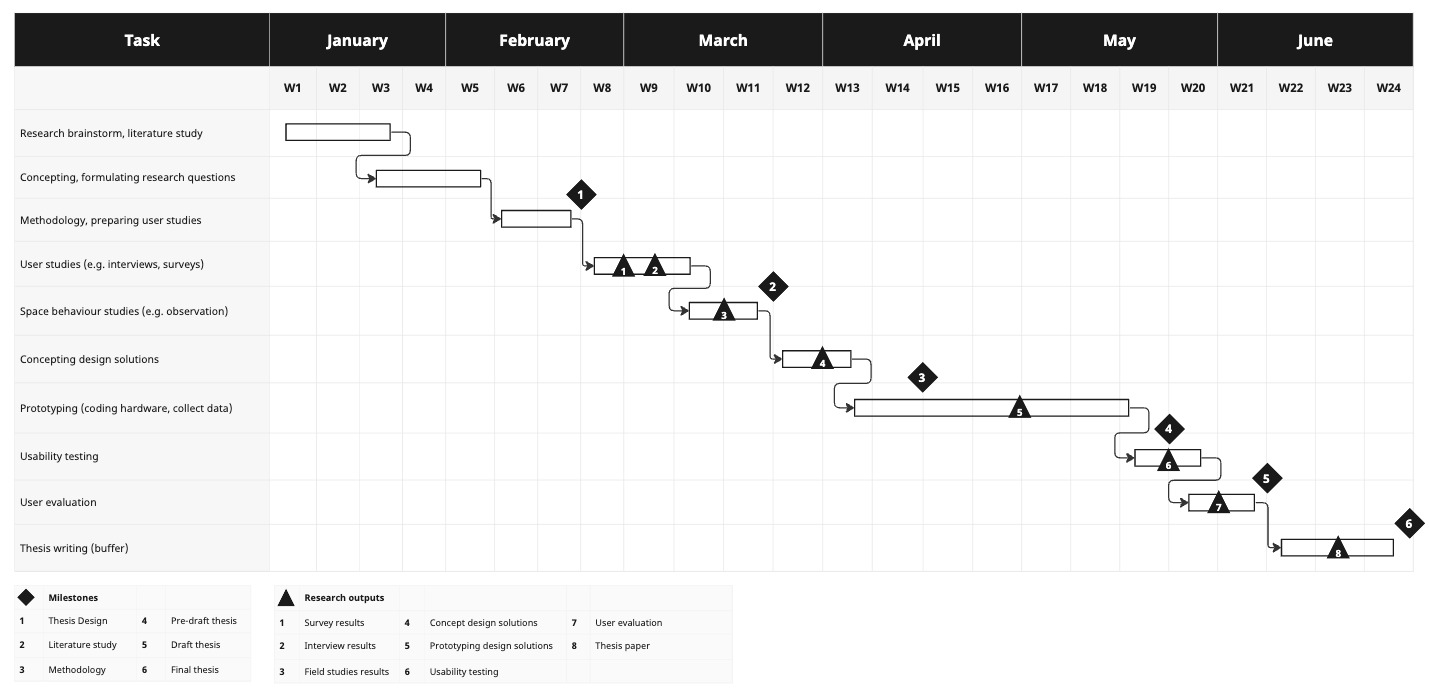
\includegraphics[width=0.71\paperwidth]{project-timeline.jpg}
    \caption{Project timeline that shows the weekly schedule}
    \label{fig:timeline}
\end{figure}

\section{Building impressions}
\label{appendix:building}

\begin{figure}[H]
    \centering
    \captionsetup{justification=centering}
    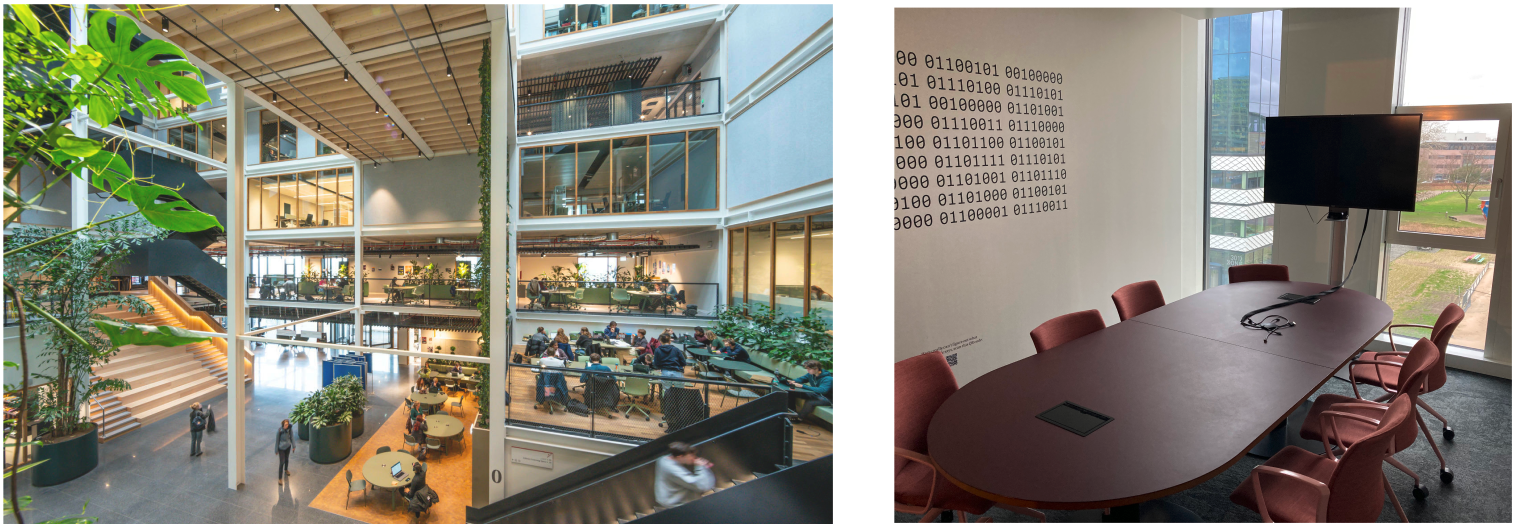
\includegraphics[width=0.686\paperwidth]{building-impressions.jpg}
    \caption{Photographs for impressions of the Lab42 building}
    \label{fig:building}
\end{figure}

\end{appendices}